\section{Two-body problem with point mass moving in a Keplerian orbit about the Earth}\label{sec:q2}

Given is:

%===========================================
\begin{equation}
    r = \frac{p}{1 + e\cos{\theta}}
    \tag{2.3\cite{wakker}}
    \label{eq:q2_1}
\end{equation}
%===========================================








\noindent \textbf{a) Derive from Equation \ref{eq:q2_1} the following equations for the velocity components $\dot{r}$ and $r\dot{\theta}$.}

\bigskip

\noindent \textit{This derivation is performed in \cite{wakker} page 119, 125 and 135.}

\bigskip

\noindent First the radial component is determined. It is known that:

%===========================================
\begin{equation}
    p = \frac{H^2}{\mu}; \hspace{0.25cm} H = r^2 \dot{\theta}
    \tag{5.21\cite{wakker}}
    \label{eq:q2_p}
\end{equation}
%===========================================

\noindent Equation \ref{eq:q2_1} becomes:

%===========================================
\begin{equation}
    r = \frac{H^2}{\mu}\frac{1}{1 + e\cos{\theta}}
    \tag{2.22\cite{wakker}}
    \label{eq:q2_2}
\end{equation}
%===========================================

\noindent Taking the time derivative of Equation \ref{eq:q2_2}:

%===========================================
\begin{equation}
    \dot{r} = \frac{H^2}{\mu}\bigg( \frac{1}{1 + e\cos{\theta}} \bigg)' = \frac{H^2}{\mu} \frac{1}{(1 + e\cos{\theta})^2} (1 + e\cos{\theta})' = \frac{H^2}{\mu} \frac{e\sin{\theta}}{(1 + e\cos{\theta})^2} \dot{\theta} 
    \tag{2.26\cite{wakker}}
    \label{eq:q2_3}
\end{equation}
%===========================================

\noindent Implement Equation \ref{eq:q2_2} for $r$ in Equation \ref{eq:q2_3}:

%===========================================
\begin{equation}
    \dot{r} = \frac{H^2}{\mu} \frac{e\sin{\theta}}{(1 + e\cos{\theta})^2} \frac{H}{r^2} 
    \label{eq:q2_4}
\end{equation}
%===========================================

\noindent Implement Equation \ref{eq:q2_p} for $\dot{\theta}$ in Equation \ref{eq:q2_4} gives the final result:

%===========================================
\begin{equation}
    \dot{r} = \frac{H^3}{\mu} \frac{e\sin{\theta}}{(1 + e\cos{\theta})^2} \frac{\mu^2(1 + e\cos{\theta})^2}{H^4} = \boldsymbol{\frac{\mu}{H} e\sin(\theta)}
    \tag{2.26\cite{wakker}}
    \label{eq:q2_5}
\end{equation}
%===========================================

\noindent Now the normal component is determined. Rearranging Equation \ref{eq:q2_p} for $r\dot{\theta}$ and replacing $r$ by using Equation \ref{eq:q2_2} gives the final result:

%===========================================
\begin{equation}
    r\dot{\theta} = \frac{H}{r} = H \frac{\mu}{H^2} (1 + e\cos{\theta}) = \boldsymbol{\frac{\mu}{H}(1 + e\cos{\theta})}
    \tag{2.27\cite{wakker}}
    \label{eq:q2_6}
\end{equation}
%===========================================










\noindent \textbf{b) Derive the equation of the velocity hodograph that expresses the relation between $\dot{r}$ and $r\dot{\theta}$. Draw for an elliptical, parabolic and hyperbolic orbit such a velocity hodograph. Indicate in these sketches the position of perigee and apogee, the true anomaly $\theta$, the eccentricity $e$, the quantity $\gamma_{max}$ and the quantity $\theta_{lim}$ for a hyperbola.}

\bigskip

\noindent \textit{This derivation is performed in \cite{wakker} page 136.}

\bigskip

\noindent To express the relation between $\dot{r}$ and $r\dot{\theta}$, $\theta$ is eliminated from Equations \ref{eq:q2_5} and \ref{eq:q2_6} by taking the quadratic of those, adding up and rearranging such that the right hand side becomes $(\frac{\mu e}{H})^2$:

%===========================================
\begin{equation}
    \dot{r}^2 + (r\dot{\theta} - \frac{\mu}{H})^2 = (\frac{\mu}{H} e\sin{\theta})^2 + (\frac{\mu}{H} e\cos{\theta})^2 = (\frac{\mu}{H}e)^2 (\sin{\theta}^2 + \cos{\theta}^2) = \boldsymbol{(\frac{\mu}{H}e)^2}
    \tag{2.27\cite{wakker}}
    \label{eq:q2_7}
\end{equation}
%===========================================

\noindent The sketches of the velocity hodographs are shown below.

%===========================================
\begin{figure}[ht]
    \centering
    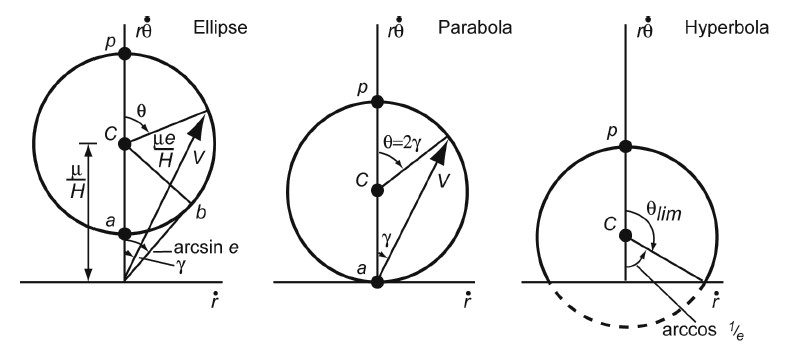
\includegraphics[width=14cm]{img/velhodo.jpg}
    \label{fig:velhodo}
\end{figure}
%===========================================








\noindent \textbf{c) Derive the relations (Whittaker's theorem) for the velocity components $V_{l}$ and $V_{n}$}

\bigskip

\noindent \textit{This derivation is performed in \cite{wakker} page 137.}

\bigskip

\noindent From Figure \ref{fig:q2c}, $V_{l}$ and $V_{n}$ can be determined:

%===========================================
\begin{equation}
    V_{l} = \frac{\dot{r}}{\sin{(\pi - \theta)}} = \frac{\dot{r}}{\sin{\theta}}   
    \label{eq:q2_8}
\end{equation}
%===========================================

%===========================================
\begin{equation}
    V_{n} = r\dot{\theta} + x = r\dot{\theta} + \frac{\dot{r}}{\tan{(\pi - \theta)}} = r\dot{\theta} - \frac{\dot{r}}{\tan{(\theta)}}
    \label{eq:q2_9}
\end{equation}
%===========================================

%===========================================
\begin{figure}[ht]
    \centering
    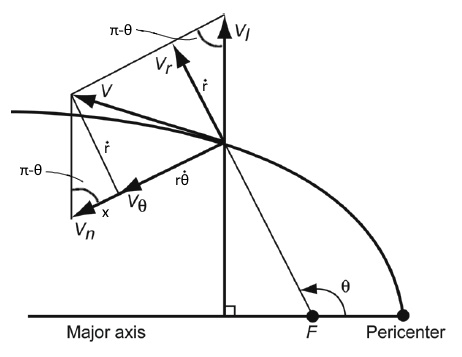
\includegraphics[width=8cm]{img/q2c.jpg}
    \caption{Definition of the velocity components $V_{l}$ and $V_{n}$. \textit{This is Figure 5.8 in \cite{wakker}.}}
    \label{fig:q2c}
\end{figure}
%===========================================

\noindent Implement Equations \ref{eq:q2_5} and \ref{eq:q2_6} in Equations \ref{eq:q2_8} and \ref{eq:q2_9}:

%===========================================
\begin{equation}
    V_{l} = \frac{\frac{\mu}{H} e\sin(\theta)}{\sin{\theta}} = \boldsymbol{\frac{\mu e}{H}}
    \tag{5.30a\cite{wakker}}
    \label{eq:q2_10}
\end{equation}
%===========================================

%===========================================
\begin{equation}
    V_{n} = \frac{\mu}{H}(1 + e\cos{\theta}) - \frac{\frac{\mu}{H} e\sin(\theta)}{\tan{(\theta)}} = \frac{\mu}{H} + \frac{\mu}{H}(e\cos{\theta}) - \frac{\frac{\mu}{H} e\sin(\theta)}{\frac{\sin{\theta}}{\cos{\theta}}} = \frac{\mu}{H} + \frac{\mu}{H}(e\cos{\theta}) - \frac{\mu}{H}e\cos(\theta) = \boldsymbol{\frac{\mu}{H}}
    \tag{5.30b\cite{wakker}}
    \label{eq:q2_11}
\end{equation}
%===========================================










\noindent \textbf{d) Use these equations to show that for an elliptical orbit the (total) velocities at perigee and at apogee are oriented perpendicular to the axis of symmetry of the conic section, and that at perigee the velocity is larger than at apogee.}

\bigskip

\noindent \textit{This information is sourced from \cite{wakker} page 137.}

\bigskip

\noindent Equations \ref{eq:q2_10} and \ref{eq:q2_11} are constant values, meaning the magnitude of these velocity components are constant for a Keplerian orbit. Also, $V_{l}$ has a constant direction. At pericenter passage, both velocity components have the same direction, resulting in a maximum value for the velocity. At apocenter passage, $V_{n}$ is directed opposite to $V_{l}$, resulting in a minimum value for the velocity. This is shown in Figure \ref{fig:whittaker} below. From this figure, one can also observe that the velocity components at perigee and apogee are oriented perpendicular with the axis of symmetry.

%===========================================
\begin{figure}[ht]
    \centering
    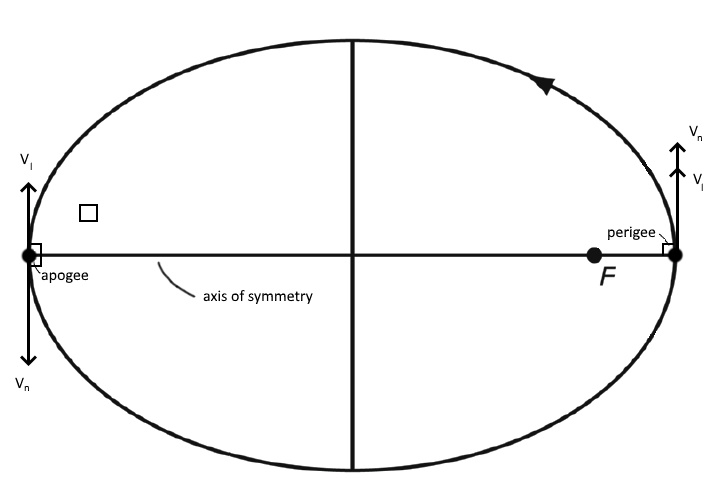
\includegraphics[width=8cm]{img/whittaker.jpg}
    \caption{Velocity components at perigee and apogee.}
    \label{fig:whittaker}
\end{figure}
%===========================================











\noindent \textbf{e) (i) Derive for an elliptical orbit the following expression for the difference between the velocity at perigee and the velocity at apogee.}

\bigskip

\noindent \textit{This information is sourced from \cite{wakker} page 163.}

\bigskip

\noindent Given is:

%===========================================
\begin{equation}
    \Delta V = V_{p} - V_{a}
    \label{eq:q2_e1}
\end{equation}
%===========================================

\noindent From \cite{wakker} the following equations for perigee and apogee velocity are sourced respectively:

%===========================================
\begin{equation}
    V_{p}^2 = V_{c_{p}}^2 (1 + e)
    \tag{6.23\cite{wakker}}
    \label{eq:q2_e2}
\end{equation}
%===========================================

%===========================================
\begin{equation}
    \frac{V_{p}}{V_{a}} = \frac{1 + e}{1 - e}
    \tag{6.24\cite{wakker}}
    \label{eq:q2_e3}
\end{equation}
%===========================================

\noindent Rearranging Equations \ref{eq:q2_e2} and \ref{eq:q2_e3}:

%===========================================
\begin{equation}
    V_{p} = V_{c_{p}} \sqrt{1 + e}
    \label{eq:q2_e4}
\end{equation}
%===========================================

%===========================================
\begin{equation}
    V_{a} = V_{p} \frac{1 - e}{1 + e}
    \label{eq:q2_e5}
\end{equation}
%===========================================

\noindent Substituting in Equation \ref{eq:q2_e1} gives the final result for an elliptical orbit:

%===========================================
\begin{multline}
    \Delta V = V_{c_{p}} \sqrt{1 + e} - \boldsymbol{V_{p}} \frac{1 - e}{1 + e} 
    = V_{c_{p}} \sqrt{1 + e} - V_{c_{p}} \sqrt{1 + e} \frac{1 - e}{1 + e} 
    = V_{c_{p}} \sqrt{1 +e} \Bigg( 1 - \frac{1 - e}{1 + e} \Bigg) \\
    = V_{c_{p}} \sqrt{1 +e} \Bigg( \frac{1 + e - (1 - e)}{1 + e} \Bigg)
    = V_{c_{p}} \sqrt{1 +e} \frac{2e}{1 + e}
    = \boldsymbol{2V_{c_{p}} \frac{e}{\sqrt{1 + e}}}
    \label{eq:q2_e6}
\end{multline}
%===========================================

\noindent \textbf{e) (ii) Derive an expression for this velocity difference if $e > 1$ and give a physical interpretation of the result obtained.}

\bigskip

\noindent \textit{This information is sourced from \cite{wakker} page 193.}

\bigskip

\noindent If $e > 1$, a hyperbolic orbit is present. The following equations for perigee and apogee velocity are sourced respectively from \cite{wakker}. A hyperbolic orbit has no apogee, a minimum velocity reaches a minimum when $r = \infty$:

%===========================================
\begin{equation}
    V_{p}^2 = V_{c_{p}}^2 (1 + e)
    \tag{8.11\cite{wakker}}
    \label{eq:q2_e7}
\end{equation}
%===========================================

%===========================================
\begin{equation}
    \frac{V_{p}}{V_{\infty}} = \sqrt{\frac{1 + e}{1 - e}}
    \tag{8.13\cite{wakker}}
    \label{eq:q2_e8}
\end{equation}
%===========================================

\noindent Rearranging Equations \ref{eq:q2_e7} and \ref{eq:q2_e8}:

%===========================================
\begin{equation}
    V_{p} = V_{c_{p}} \sqrt{1 + e}
    \label{eq:q2_e9}
\end{equation}
%===========================================

%===========================================
\begin{equation}
    V_{\infty} = V_{p} \sqrt{\frac{1 - e}{1 + e}}
    \label{eq:q2_e10}
\end{equation}
%===========================================

\noindent Substituting in Equation \ref{eq:q2_e1} gives the final result for a hyperbolic orbit:

%===========================================
\begin{multline}
    \Delta V = V_{p} - V_{\infty} = V_{c_{p}} \sqrt{1 + e} - V_{p} \sqrt{\frac{1 - e}{1 + e}}
    = V_{c_{p}} \sqrt{1 + e} - V_{c_{p}} \sqrt{1 + e} \sqrt{\frac{1 - e}{1 + e}} \\
    = V_{c_{p}} \sqrt{1 + e} - V_{c_{p}} \sqrt{1 - e}
    = \boldsymbol{V_{c_{p}} \bigg( \sqrt{1 + e} - \sqrt{1 - e} \bigg)}
    \label{eq:q2_final}
\end{multline}
%===========================================

\noindent When the eccentricity of a hyperbolic orbit increases from somewhere between 1 and 1.25, the $\Delta V$ becomes larger. From $e > 1.25$, the $\Delta V$ decreases.